\documentclass[12pt]{report}
\usepackage[utf8]{inputenc}
\usepackage[russian]{babel}
%\usepackage[14pt]{extsizes}
\usepackage{listings}
\usepackage{graphicx}
\usepackage{amsmath,amsfonts,amssymb,amsthm,mathtools} 
\usepackage{pgfplots}
\usepackage{filecontents}
\usepackage{float}
\usepackage{comment}
\usepackage{indentfirst}
\usepackage{eucal}
\usepackage{enumitem}
%s\documentclass[openany]{book}
\frenchspacing

\usepackage{array}

\usepackage{verbatim}

\usepackage{caption}
\captionsetup{labelsep=endash}
\captionsetup[figure]{name={Рисунок}}

\usepackage{indentfirst} % Красная строка

\usetikzlibrary{datavisualization}
\usetikzlibrary{datavisualization.formats.functions}

\usepackage{amsmath}


% Для листинга кода:
\lstset{ %
	language=c,                 % выбор языка для подсветки (здесь это С)
	basicstyle=\small\sffamily, % размер и начертание шрифта для подсветки кода
	numbers=left,               % где поставить нумерацию строк (слева\справа)
	numberstyle=\tiny,           % размер шрифта для номеров строк
	stepnumber=1,                   % размер шага между двумя номерами строк
	numbersep=5pt,                % как далеко отстоят номера строк от подсвечиваемого кода
	showspaces=false,            % показывать или нет пробелы специальными отступами
	showstringspaces=false,      % показывать или нет пробелы в строках
	showtabs=false,             % показывать или нет табуляцию в строках
	frame=single,              % рисовать рамку вокруг кода
	tabsize=2,                 % размер табуляции по умолчанию равен 2 пробелам
	captionpos=t,              % позиция заголовка вверху [t] или внизу [b] 
	breaklines=true,           % автоматически переносить строки (да\нет)
	breakatwhitespace=false, % переносить строки только если есть пробел
	escapeinside={\#*}{*)}   % если нужно добавить комментарии в коде
}


\usepackage[left=2cm,right=2cm, top=2cm,bottom=2cm,bindingoffset=0cm]{geometry}
% Для измененных титулов глав:
\usepackage{titlesec, blindtext, color} % подключаем нужные пакеты
\definecolor{gray75}{gray}{0.75} % определяем цвет
\newcommand{\hsp}{\hspace{20pt}} % длина линии в 20pt
% titleformat определяет стиль
\titleformat{\chapter}[hang]{\Huge\bfseries}{\thechapter\hsp\textcolor{gray75}{|}\hsp}{0pt}{\Huge\bfseries}


% plot
\usepackage{pgfplots}
\usepackage{filecontents}
\usetikzlibrary{datavisualization}
\usetikzlibrary{datavisualization.formats.functions}

\begin{document}
	%\def\chaptername{} % убирает "Глава"
	\thispagestyle{empty}
	\begin{titlepage}
		\noindent \begin{minipage}{0.15\textwidth}
			
\includegraphics[width=\linewidth]{inc/b_logo}
		\end{minipage}
		\noindent\begin{minipage}{0.9\textwidth}\centering
			\textbf{Министерство науки и высшего образования Российской Федерации}\\
			\textbf{Федеральное государственное бюджетное образовательное учреждение высшего образования}\\
			\textbf{~~~«Московский государственный технический университет имени Н.Э.~Баумана}\\
			\textbf{(национальный исследовательский университет)»}\\
			\textbf{(МГТУ им. Н.Э.~Баумана)}
		\end{minipage}
		
		\noindent\rule{18cm}{3pt}
		\newline\newline
		\noindent ФАКУЛЬТЕТ $\underline{\text{«Информатика и системы управления»}}$ \newline\newline
		\noindent КАФЕДРА $\underline{\text{«Программное обеспечение ЭВМ и информационные технологии»}}$\newline\newline\newline\newline\newline
		
		\begin{center}
			\noindent\begin{minipage}{1.1\textwidth}\centering
				\Large\textbf{Отчет по лабораторной работе №5}\newline
				\textbf{по дисциплине <<Моделирование>>}\newline\newline
			\end{minipage}
		\end{center}
		
		\noindent\textbf{Тема} $\underline{\text{Моделирование информационного центра}}$\newline\newline
		\noindent\textbf{Студент} $\underline{\text{Слепокурова М.Ф.}}$\newline\newline
		\noindent\textbf{Группа} $\underline{\text{ИУ7-76Б}}$\newline\newline
		\noindent\textbf{Оценка (баллы)} $\underline{\text{~~~~~~~~~~~~~~~~~}}$\newline\newline
		\noindent\textbf{Преподаватель} $\underline{\text{Рудаков И.В.}}$\newline\newline\newline
		
		\begin{center}
			\vfill
			Москва~---~\the\year
			~г.
		\end{center}
	\end{titlepage}

\setcounter{page} {2}


\section*{Постановка задачи}
В информационный центр приходят клиенты через интервалы времени $10 \pm 2$ минуты. Если все три имеющихся оператора заняты, клиенту отказывают в обслуживании. Операторы имеют разную производительность и могут обеспечивать обслуживание среднего запроса пользователя за $20 \pm 5$, $40 \pm 10$, $40 \pm 20$ минут. Клиенты стремятся занять свободного оператора с максимальной производительностью. Полученные запросы сдаются в приемный накопитель, откуда они выбираются для обработки. На первый компьютер — запросы от первого и второго оператора, на второй компьютер — от третьего оператора. Время обработки на первом и втором компьютере равны соответственно 15 и 30 минутам. За единицу системного времени выбрать 0.01 минуты.

В процессе взаимодействия клиентов и центра возможны: режим нормального обслуживания (клиент выбирает одного из свободных операторов, но предпочитает того, у которого номер меньше) и режим отказа.


В рамках поставленной задачи необходимо:
\begin{itemize}
    \item смоделировать процесс обработки 300 запросов;
    \item определить вероятность отказа;
    \item построить структурную схему модели;
    \item нарисовать модель в терминах СМО.
\end{itemize}

\section*{Теория}

\subsection*{Анализ задачи}
Эндогенные переменные: время обработки задания $i$-м оператором и время решения задания на $j$-м компьютере.

Экзогенные переменные: $n_0$ --- число обслуженных клиентов, $n_1$ --- число клиентов, получивших отказ.

Вероятность отказа может быть рассчитана по следующей формуле:
$\frac{n_1}{n_0 + n_1}$.

На рисунке \ref{img:schema1} изображена структурная схема реализуемой модели.

\begin{figure}[h!btp]
	\centering
	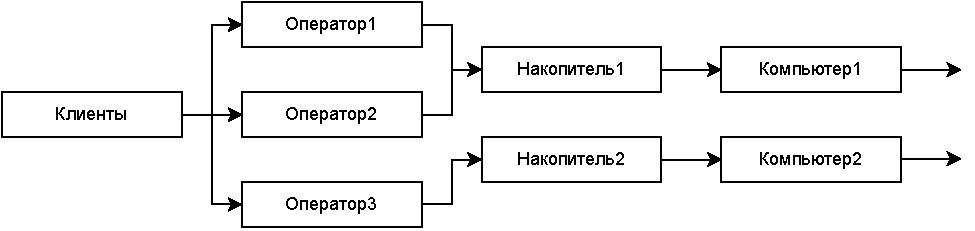
\includegraphics[width=1\columnwidth]{inc/schema1.pdf}
	\caption{Структурная схема модели}
	\label{img:schema1}	
\end{figure}


На рисунке \ref{img:schema2} изображена схема модели в терминах СМО, где $\text{Г}$ --- генератор заявок, $\text{К}_i$ --- канал обработки, $\text{Н}_i$ --- накопитель.

\begin{figure}[h!btp]
	\centering
	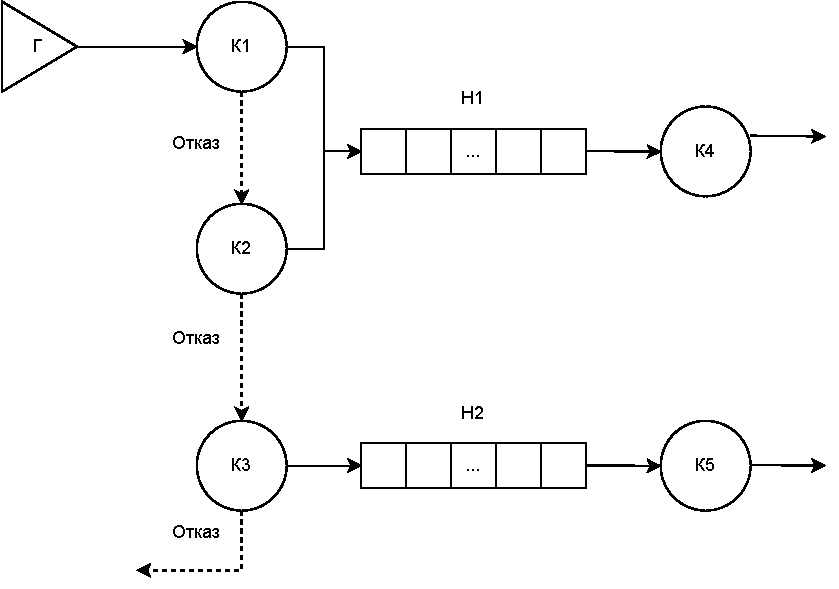
\includegraphics[width=0.8\columnwidth]{inc/schema2.pdf}
	\caption{Схема модели в терминах СМО}
	\label{img:schema2}	
\end{figure}

\subsection*{Принцип $\Delta t$}
Данный принцип заключается в последовательном анализе состояний всех блоков в момент $t + \Delta t$ по заданному состоянию блоков в момент времени $t$, при этом новое состояние блоков определяется в соответствии с их алгоритмическим описанием с учетом действующих случайных факторов, задаваемых распределениями вероятности. В результате такого анализа принимается решение о том, какие общесистемные события должны имитироваться программной моделью на данный момент времени.

\section*{Средства реализации}

Для реализации приложения был выбран язык программирования Python.

\clearpage
\section*{Листинг кода}

\begin{lstlisting}
from numpy.random import uniform

class TimeGenerator:
  def __init__(self, time, delta):
    self.time = time
    self.delta = delta

  def randomTime(self):
    return uniform(self.time - self.delta, self.time + self.delta)

class RequestGenerator:
  def __init__(self, timeGenerator, count, recievers = []):
    self.timeGenerator = timeGenerator
    self.requestCount = count
    self.receivers = recievers
    self.next = 0

  def generateRequest(self, currTime):
    self.requestCount -= 1
    self.next = currTime + self.generateDuration()
    for receiver in self.receivers:
      if not receiver.busy: return receiver
    return None

  def generateDuration(self):
    return self.timeGenerator.randomTime()

class RequestOperator:
  def __init__(self, timeGenerator, processor):
    self.timeGenerator = timeGenerator
    self.next = 0
    self.processor = processor
    self.busy = False

  def receiveRequest(self, currTime):
    self.busy = True
    self.next = currTime + self.generateDuration()

  def processRequest(self):
    if self.busy:
      self.next = 0
      self.busy = False

  def generateDuration(self):
    return self.timeGenerator.randomTime()
\end{lstlisting}
\clearpage
\begin{lstlisting}
class RequestProcessor:
  def __init__(self, timeGenerator):
    self.timeGenerator = timeGenerator
    self.queueSize = 0
    self.next = 0

  def pushRequest(self):
    self.queueSize += 1

  def popRequest(self, currTime):
    if self.queueSize > 0:
      self.queueSize -= 1
      self.next = currTime + self.generateDuration()
    else:
      self.next = 0

  def generateDuration(self):
    return self.timeGenerator.randomTime()

class Model:
  def __init__(self, generator, operators, processors):
    self.generator = generator
    self.operators = operators
    self.processors = processors

  def simulate(self, delta):
    refusalCount = 0
    generatedRequests = self.generator.requestCount
    blocks = [self.generator, *self.operators, *self.processors]
    
    currTime = 0
    while self.generator.requestCount > 0:
      for block in blocks:
        if block.next <= currTime:
          if isinstance(block, RequestGenerator):
            receiver = self.generator.generateRequest(currTime)
            if not receiver: refusalCount += 1
            else: receiver.receiveRequest(currTime)
          elif isinstance(block, RequestOperator):
            block.processRequest()
            block.processor.pushRequest()
          elif isinstance(block, RequestProcessor):
            block.popRequest(currTime)
      currTime += delta
      
    return { "refusalProbability": refusalCount / generatedRequests, "refusalCount": refusalCount }

requestCount = 300
\end{lstlisting}
\clearpage
\begin{lstlisting}
computer1 = RequestProcessor(TimeGenerator(15, 0))
computer2 = RequestProcessor(TimeGenerator(30, 0))

operator1 = RequestOperator(TimeGenerator(20, 5), computer1)
operator2 = RequestOperator(TimeGenerator(40, 10), computer1)
operator3 = RequestOperator(TimeGenerator(40, 20), computer2)

requestGenerator = RequestGenerator(TimeGenerator(10, 2), requestCount, [operator1, operator2, operator3])

model = Model(requestGenerator, [operator1, operator2, operator3], [computer1, computer2])
result = model.simulate(0.01)

refusalCount, refusalProbability = result["refusalCount"], result["refusalProbability"]

print("Requests: ", requestCount)
print("Refusals: ", refusalCount)
print("Refusal probability: ", round(refusalProbability, 2))
\end{lstlisting}


\section*{Демонстрация работы программы}
На рисунке \ref{fig:pic1} изображен пример работы программы для 300 заявок.

\begin{figure}[h!btp]
	\centering
	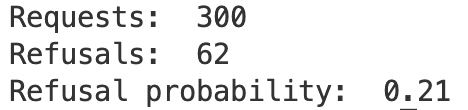
\includegraphics[width=0.4\textwidth]{inc/pic1.png}
	\caption{Пример работы программы --- 1}
	\label{fig:pic1}	
\end{figure}

На рисунке \ref{fig:pic2} изображен пример работы программы для 500 заявок.

\begin{figure}[h!btp]
	\centering
	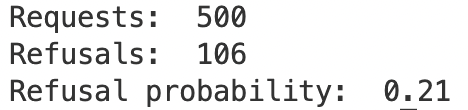
\includegraphics[width=0.4\textwidth]{inc/pic2.png}
	\caption{Пример работы программы --- 2}
	\label{fig:pic2}	
\end{figure}

На рисунке \ref{fig:pic3} изображен пример работы программы для 1000 заявок.

\begin{figure}[h!btp]
	\centering
	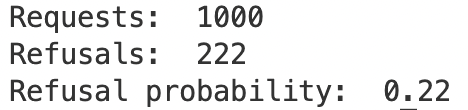
\includegraphics[width=0.4\textwidth]{inc/pic3.png}
	\caption{Пример работы программы --- 3}
	\label{fig:pic3}	
\end{figure}

\bibliographystyle{utf8gost705u}  % стилевой файл для оформления по ГОСТу
\bibliography{51-biblio}          % имя библиографической базы (bib-файла)
	
\end{document}
